% Options for packages loaded elsewhere
\PassOptionsToPackage{unicode}{hyperref}
\PassOptionsToPackage{hyphens}{url}
%
\documentclass[
  11pt,
]{article}
\usepackage{amsmath,amssymb}
\usepackage{iftex}
\ifPDFTeX
  \usepackage[T1]{fontenc}
  \usepackage[utf8]{inputenc}
  \usepackage{textcomp} % provide euro and other symbols
\else % if luatex or xetex
  \usepackage{unicode-math} % this also loads fontspec
  \defaultfontfeatures{Scale=MatchLowercase}
  \defaultfontfeatures[\rmfamily]{Ligatures=TeX,Scale=1}
\fi
\usepackage{lmodern}
\ifPDFTeX\else
  % xetex/luatex font selection
\fi
% Use upquote if available, for straight quotes in verbatim environments
\IfFileExists{upquote.sty}{\usepackage{upquote}}{}
\IfFileExists{microtype.sty}{% use microtype if available
  \usepackage[]{microtype}
  \UseMicrotypeSet[protrusion]{basicmath} % disable protrusion for tt fonts
}{}
\makeatletter
\@ifundefined{KOMAClassName}{% if non-KOMA class
  \IfFileExists{parskip.sty}{%
    \usepackage{parskip}
  }{% else
    \setlength{\parindent}{0pt}
    \setlength{\parskip}{6pt plus 2pt minus 1pt}}
}{% if KOMA class
  \KOMAoptions{parskip=half}}
\makeatother
\usepackage{xcolor}
\usepackage[margin=0.5in]{geometry}
\usepackage{longtable,booktabs,array}
\usepackage{calc} % for calculating minipage widths
% Correct order of tables after \paragraph or \subparagraph
\usepackage{etoolbox}
\makeatletter
\patchcmd\longtable{\par}{\if@noskipsec\mbox{}\fi\par}{}{}
\makeatother
% Allow footnotes in longtable head/foot
\IfFileExists{footnotehyper.sty}{\usepackage{footnotehyper}}{\usepackage{footnote}}
\makesavenoteenv{longtable}
\usepackage{graphicx}
\makeatletter
\def\maxwidth{\ifdim\Gin@nat@width>\linewidth\linewidth\else\Gin@nat@width\fi}
\def\maxheight{\ifdim\Gin@nat@height>\textheight\textheight\else\Gin@nat@height\fi}
\makeatother
% Scale images if necessary, so that they will not overflow the page
% margins by default, and it is still possible to overwrite the defaults
% using explicit options in \includegraphics[width, height, ...]{}
\setkeys{Gin}{width=\maxwidth,height=\maxheight,keepaspectratio}
% Set default figure placement to htbp
\makeatletter
\def\fps@figure{htbp}
\makeatother
\setlength{\emergencystretch}{3em} % prevent overfull lines
\providecommand{\tightlist}{%
  \setlength{\itemsep}{0pt}\setlength{\parskip}{0pt}}
\setcounter{secnumdepth}{-\maxdimen} % remove section numbering
% definitions for citeproc citations
\NewDocumentCommand\citeproctext{}{}
\NewDocumentCommand\citeproc{mm}{%
  \begingroup\def\citeproctext{#2}\cite{#1}\endgroup}
\makeatletter
 % allow citations to break across lines
 \let\@cite@ofmt\@firstofone
 % avoid brackets around text for \cite:
 \def\@biblabel#1{}
 \def\@cite#1#2{{#1\if@tempswa , #2\fi}}
\makeatother
\newlength{\cslhangindent}
\setlength{\cslhangindent}{1.5em}
\newlength{\csllabelwidth}
\setlength{\csllabelwidth}{3em}
\newenvironment{CSLReferences}[2] % #1 hanging-indent, #2 entry-spacing
 {\begin{list}{}{%
  \setlength{\itemindent}{0pt}
  \setlength{\leftmargin}{0pt}
  \setlength{\parsep}{0pt}
  % turn on hanging indent if param 1 is 1
  \ifodd #1
   \setlength{\leftmargin}{\cslhangindent}
   \setlength{\itemindent}{-1\cslhangindent}
  \fi
  % set entry spacing
  \setlength{\itemsep}{#2\baselineskip}}}
 {\end{list}}
\usepackage{calc}
\newcommand{\CSLBlock}[1]{\hfill\break#1\hfill\break}
\newcommand{\CSLLeftMargin}[1]{\parbox[t]{\csllabelwidth}{\strut#1\strut}}
\newcommand{\CSLRightInline}[1]{\parbox[t]{\linewidth - \csllabelwidth}{\strut#1\strut}}
\newcommand{\CSLIndent}[1]{\hspace{\cslhangindent}#1}
\usepackage{hyperref}
\usepackage{array}
\usepackage{caption}
\usepackage{graphicx}
\usepackage{multirow}
\usepackage{hhline}
\usepackage{calc}
\usepackage{tabularx}
\usepackage[para,online,flushleft]{threeparttable}
\DeclareMathOperator{\logit}{logit}
\DeclareMathOperator{\var}{var}
\usepackage{float}
\ifLuaTeX
  \usepackage{selnolig}  % disable illegal ligatures
\fi
\IfFileExists{bookmark.sty}{\usepackage{bookmark}}{\usepackage{hyperref}}
\IfFileExists{xurl.sty}{\usepackage{xurl}}{} % add URL line breaks if available
\urlstyle{same}
\hypersetup{
  pdftitle={Analysis of Health Survey for England (HSE) 2019},
  pdfauthor={Candidate Numbers Here},
  hidelinks,
  pdfcreator={LaTeX via pandoc}}

\title{Analysis of Health Survey for England (HSE) 2019}
\author{Candidate Numbers Here}
\date{March 12, 2024}

\begin{document}
\maketitle
\begin{abstract}
This report provides an analysis of data related to health, age,
socio-economic factors and lifestyle habits in adults (from the age of
16) from the population in England, derived from the Health Survey for
England 2019.
\end{abstract}

\pagenumbering{gobble}

\newpage

\subsection{Summary (Non-Technical)}\label{summary-non-technical}

\subsection{Introduction}\label{introduction}

In the UK, smoking, vaping, and alcohol consumption are widespread,
particularly among youngsters. It is crucial to be aware of the
consequences and dangers of these habits, and the complications they can
cause in later-life. The Office for National Statistics (ONS), regarded
as the foremost statistical institute in the UK, is the ``go-to'' for
insights into public health trends. According to their estimations,
approximately 14.1\% of the adult population aged 18 and above were
identified as cigarette smokers (\citeproc{ref-1ONS}{ONS 2019a}).
Furthermore, their data revealed there were 7,565 deaths attributed to
alcohol-specific causes in 2019 (\citeproc{ref-2ONS}{ONS 2019b}). These
statistics alone warrant a need for an understanding of health-related
behaviours and the outcome. Therefore, the aim of our study is to
investigate not only the prevalence but also the severity of these
habits, exploring different socioeconomic factors that may potentially
contribute to each. Additionally, we will investigate the greater
implications of these bad habits and how they relate to systolic blood
pressure levels throughout the UK population.

\subsection{Exploratory Analysis}\label{exploratory-analysis}

We are using data from the 2019 Health Survey for England (HSE) to
conduct our analysis. Before proceeding with any investigations
involving the data, we checked for any common errors in large datasets.
Our initial step involved pre-processing the data, which entailed
filtering observations to include only those above the age of 16 and
removing 3 pairs of observations that were identical in every
descriptive variable except for the ID, resulting in a dataset of
\texttt{r} observations. As we have two different grouped age variables,
we ensured they were consistent with one another. \emph{Don't know if
this final sentence needs to be included}

\emph{Need the table copied over here with the variable names/a
paragraph explaining these}

We also found 36 pairs with exact entries excluding lab measurements,
but we do not remove these from our analysis. We suspect these may be
individuals who have either initially refused a nurse visit but later
changed their mind, or simply have had two nurse visits where their lab
measurements vary slightly between the two. The supporting documentation
doesn't state a protocol for repeated visits, so we will assume these
are genuine observations from different participants and include them.
\emph{Maybe rewording this?}

\emph{I think this table could be replaced with a paragraph that may
save space} All variables are coded as numeric in our dataset, so we
recoded all factor variables accordingly. Note that for the purposes of
model building, we coded CASI/CAPI responses about alcohol and cigarette
consumption in the following way:

\begin{longtable}[]{@{}
  >{\raggedright\arraybackslash}p{(\columnwidth - 6\tabcolsep) * \real{0.1264}}
  >{\raggedright\arraybackslash}p{(\columnwidth - 6\tabcolsep) * \real{0.0690}}
  >{\raggedright\arraybackslash}p{(\columnwidth - 6\tabcolsep) * \real{0.4483}}
  >{\raggedright\arraybackslash}p{(\columnwidth - 6\tabcolsep) * \real{0.3563}}@{}}
\toprule\noalign{}
\begin{minipage}[b]{\linewidth}\raggedright
Variable
\end{minipage} & \begin{minipage}[b]{\linewidth}\raggedright
Code
\end{minipage} & \begin{minipage}[b]{\linewidth}\raggedright
Label
\end{minipage} & \begin{minipage}[b]{\linewidth}\raggedright
Decode
\end{minipage} \\
\midrule\noalign{}
\endhead
\bottomrule\noalign{}
\endlastfoot
NDPNow\_19 & 1 & E-cigarettes or vaping devices only & Smokes
E-cigarettes \\
& 2 & Other nicotine delivery products only & Doesn't smoke
E-cigarettes \\
& 3 & Both & Smokes E-cigarettes \\
& 4 & None & Doesn't smoke E-cigarettes \\
& -1 & Not Applicable & NA \\
& -8 & Don't know & NA \\
& -9 & Refused & NA \\
dnoft\_19 & 1 & Almost every day & Frequently \\
& 2 & Five or six days a week & Frequently \\
& 3 & Three or four days a week & Frequently \\
& 4 & Once or twice a week & Occasionally \\
& 5 & Once or twice a month & Occasionally \\
& 6 & Once every couple of months & Rarely \\
& 7 & Once or twice a year & Rarely \\
& 8 & Not at all in the last 12 months & Rarely \\
& -1 & Not Applicable & NA \\
& -8 & Don't know & NA \\
& -9 & Refused & NA \\
\end{longtable}

We code a binary variable to group current smoking status into `yes' or
`no', with the `Ex-Reg' smokers falling into the `no' category. For
`topqual2' we group respondents into `higher education' or `basic
education' \emph{This has changed since}. Similarly, `urban14b' now has
two levels being `rural' and `urban' and `marstatD' now only has
`married' and `not married' levels.

The number of missing observations for each are shown in Table
@ref(tab:output NA table):

\begin{longtable}[]{@{}lrl@{}}
\caption{Missing values in the training dataset}\tabularnewline
\toprule\noalign{}
Variable & Missing Values & \% Missing \\
\midrule\noalign{}
\endfirsthead
\toprule\noalign{}
Variable & Missing Values & \% Missing \\
\midrule\noalign{}
\endhead
\bottomrule\noalign{}
\endlastfoot
omsysval & 2972 & 55.7\% \\
dnoft\_19 & 1097 & 20.6\% \\
topqual2 & 19 & 0.356\% \\
cigsta3\_19 & 16 & 0.3\% \\
cigdyal\_19 & 15 & 0.281\% \\
NDPNow\_19 & 14 & 0.262\% \\
d7many3\_19 & 14 & 0.262\% \\
drinkYN\_19 & 13 & 0.244\% \\
origin2 & 5 & 0.0937\% \\
marstatD & 1 & 0.0187\% \\
\end{longtable}

As expected, there is a lot of missingness in the lab values,
particularly `omsysval'. \emph{Maybe some explanation of why this is
expected?} When conducting our analysis of these, we will use a subset
including only observations with at least one of these taken. The only
other variable with a substantial amount of data missing is `dnoft\_19'
and, as this is derived from a retrospective question, this may be a
case of recall bias. Questions involving lifestyle habits such as
alcohol consumption are considered sensitive, with many individuals
potentially not being willing to answer, more likely to be the issue
here. With this level of missingness in `dnoft\_19', we decide not to
use it in any of our models. `topqual2', `origin2' and `marstatD' are
the only demographic variables with any missing entries, with 19
observations (0.356\% of the data) missing at least one. As all three of
these variables are not necessary for identifiability, we do not expect
every participant to answer these questions due to personal preference.

Finally, we analysed the two lab measurement variables in Figure
@ref(tab:output distribution plots), finding potential outliers to be
present in both. The readings for `omsysval' are collected by taking an
average of three readings, each five minutes apart, performed by a
trained nurse who deemed each reading to be valid. For this reason, it
seems highly unlikely that these readings are mistakes, and we include
them in our analysis. However, our BMI variable is estimated if the
participants weight is over 130kg. These extremely high BMI values are
most likely to be caused by the over-estimation of these participants
weights. We deem these to be errors and code them as missing in the
dataset.

\begin{figure}[H]
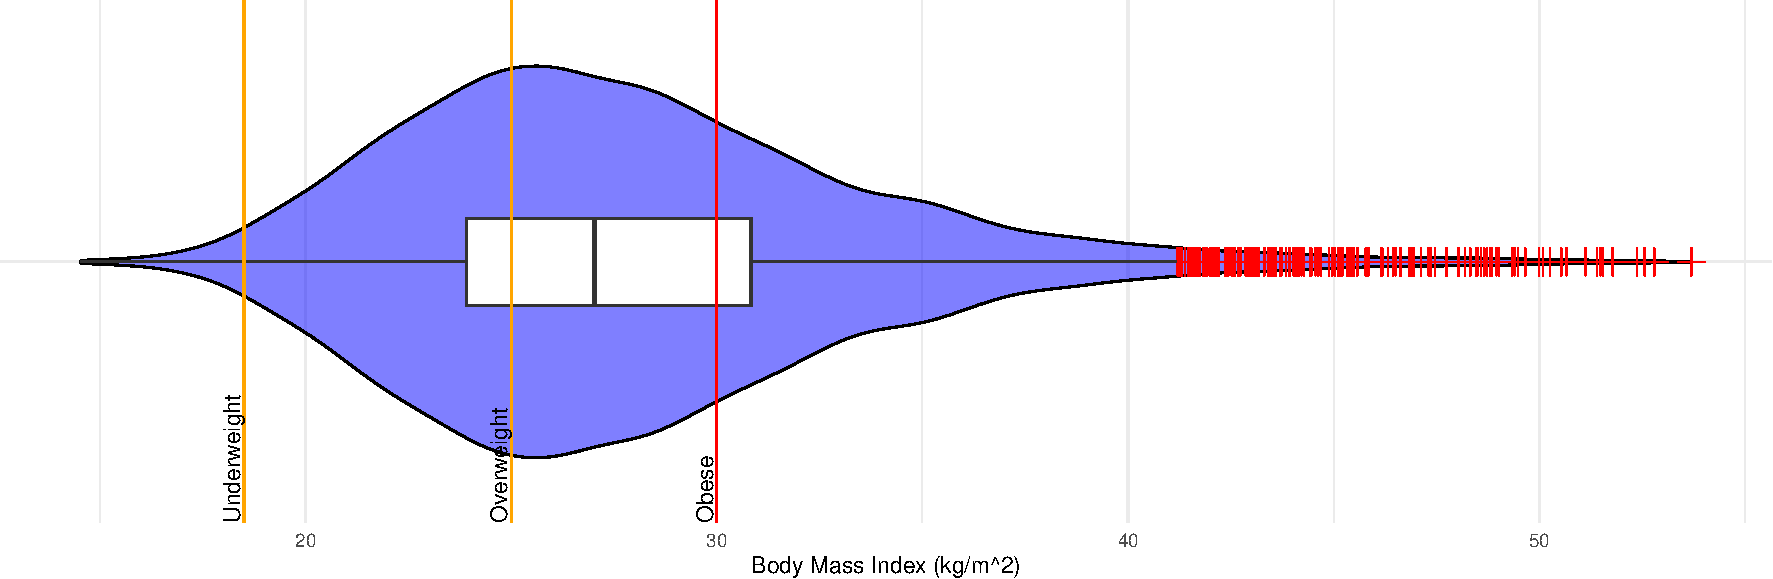
\includegraphics{Coursework_files/figure-latex/output distribution plots-1} \caption{Distribution of BMI and Mean Systolic Blood Pressure}\label{fig:output distribution plots}
\end{figure}

\subsection{Methology}\label{methology}

\subsubsection{What is the prevelance of drinking, smoking and E-cig
usage?}\label{what-is-the-prevelance-of-drinking-smoking-and-e-cig-usage}

To calculate the prevalence of each habit we assume each of the \(n\)
observations, \(x_1,…,x_n\) , to be independent, identically distributed
(iid) random variables (RVs) where
\(x_i \sim Bern(p)\, \forall i=1,…,n\) and \(p\) denotes the probability
of an observation having the relevant habit. We use the household
weights to calculate a weighted Maximum Likelihood Estimate (MLE) of
\(p\). That is, letting \(w_i\) denote the weight of the \(i^{th}\)
observation, we alter the standard likelihood function of a Bernoulli
distribution as below:
\[L(p|\textbf{x}) = \prod_{i = 1}^{n} (p^{x_i}(1-p)^{1-x_i})^{w_i}\]
From this, we calculate our weighted MLE as:
\[\widehat{p} = \frac{\sum_{i=1}^{n} x_iw_i}{\sum_{i=1}^{n} w_i}\]

It can also be shown that this MLE has variance given by
\(\mathop{\mathrm{var}}(\widehat{p})=\frac{p(1-p)}{\sum_{i=1}^{n}w_i}\),
which we can estimate using \(\widehat{p}\) and use large sample
properties of the MLE to get a normal approximation and estimate 95\%
confidence intervals for each habit, which are shown in Table
@ref(tab:output estimates table).

\begin{longtable}[]{@{}lll@{}}
\caption{Estimates and 95\% Confidence Intervals for \% of
Population}\tabularnewline
\toprule\noalign{}
Habit & Estimate & C.I. \\
\midrule\noalign{}
\endfirsthead
\toprule\noalign{}
Habit & Estimate & C.I. \\
\midrule\noalign{}
\endhead
\bottomrule\noalign{}
\endlastfoot
Drinking & 81.8\% & (80.9\%, 82.7\%) \\
Smoking & 16.7\% & (15.8\%, 17.6\%) \\
Smoking E-cigarettes & 4.4\% & (3.91\%, 4.89\%) \\
\end{longtable}

\textbf{Interpretation of table/results - e-cig is much lower, drinking
very common etc}

We segmented our data by gender, age brackets and level of deprivation
and regrouped the levels of each lifestyle factor variables into more
manageable buckets \emph{This bit should read better, but I'm not sure
the changes - just needs to be a sentence to introduce the plots}

\begin{figure}[H]
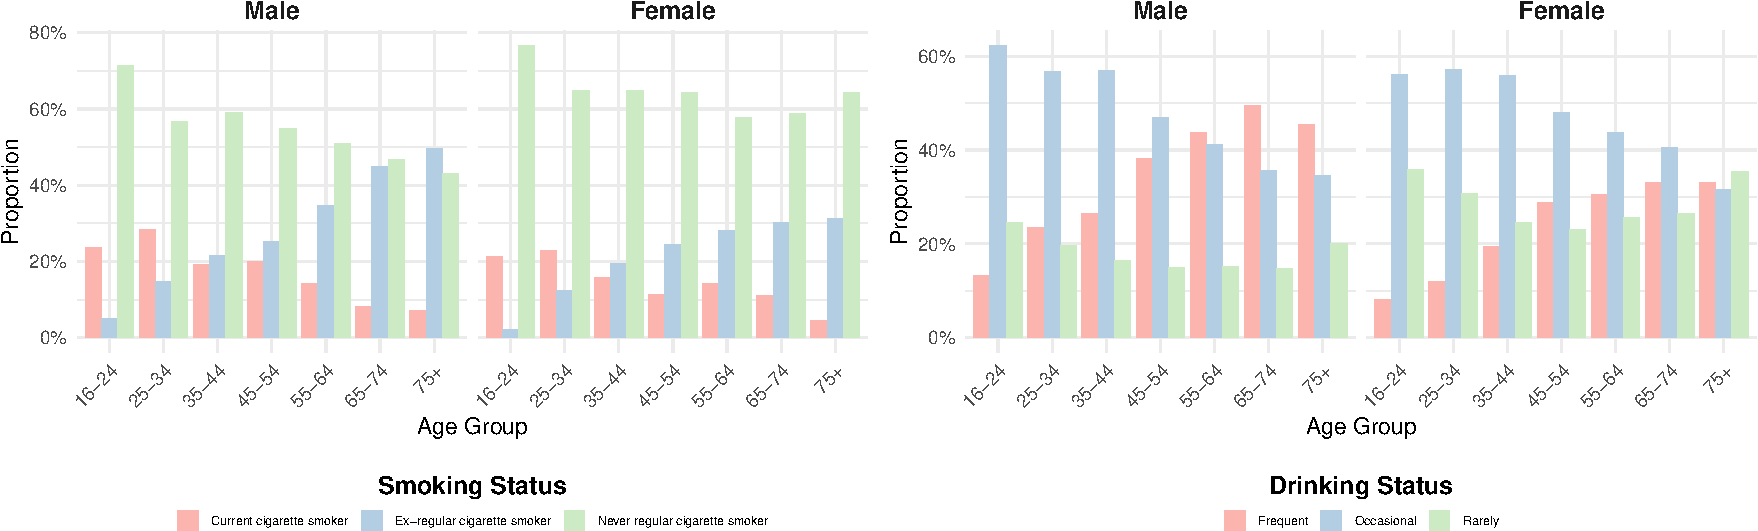
\includegraphics{Coursework_files/figure-latex/output smoking and drinking by age plot-1} \caption{Smoking and drinking status proportions by age group and gender}\label{fig:output smoking and drinking by age plot}
\end{figure}

\emph{I will change this plot to include all three (smoking, drinking,
ecigs) in one graph, similarly needs a sentence intro}

\begin{figure}[H]
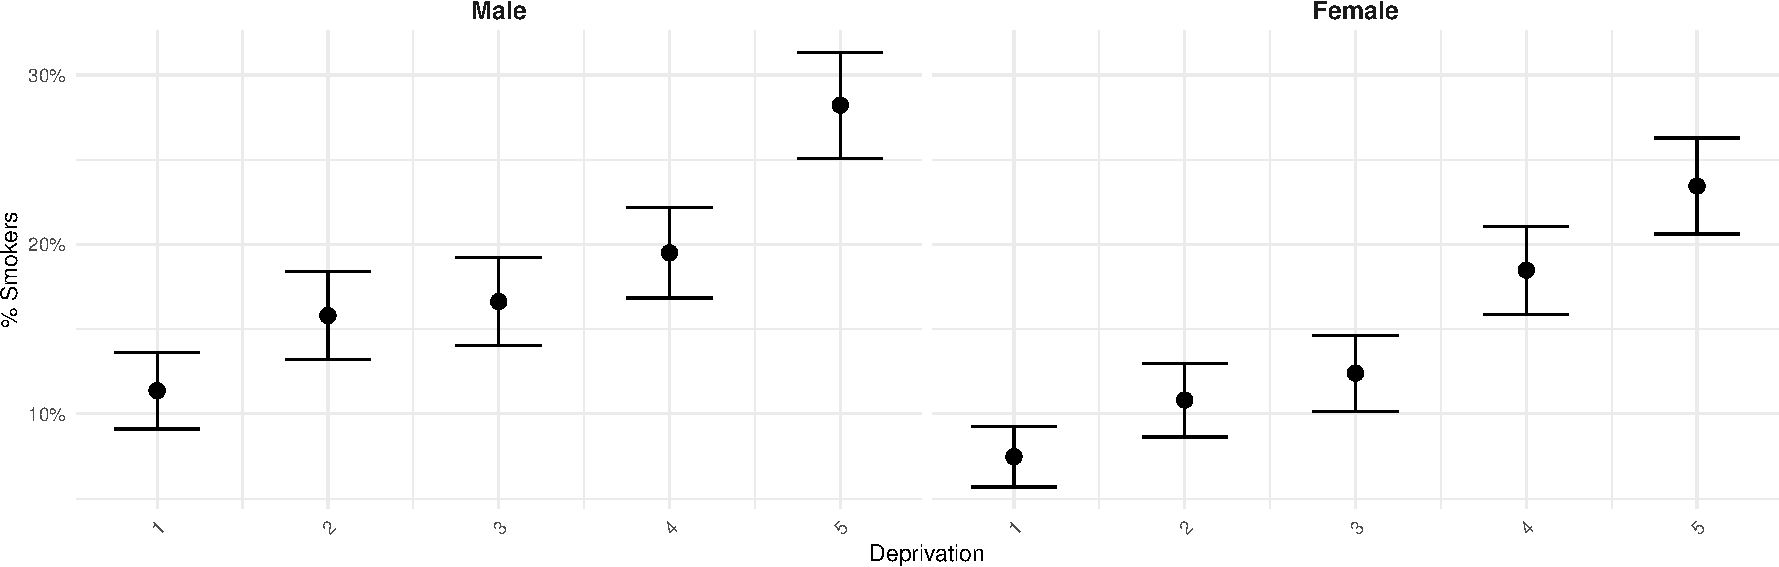
\includegraphics{Coursework_files/figure-latex/output prevelance plot-1} \caption{Estimation of the prevelance of smokers by deprivation}\label{fig:output prevelance plot}
\end{figure}

We found that the usage of e-cigarette usage among adults is relatively
low, making it challenging to dissect any significant trends within the
data. \emph{Maybe reword?} We noted an inverse correlation between age
and the proportion of `occasional' drinking, while `frequent' drinking
showed a positive correlation. Additionally, males demonstrate a higher
prevalence of drinking across nearly all demographic categories in
comparison to females. `Active' smoking appears to follow a similar
relationship to `occasional' drinkers, with the number of `active'
smokers decreasing with age. Interestingly, the proportion of males who
quit smoking in later-life is consistently greater than that of females.

\emph{This probably needs rewording} It is important to mention the
variable `Level of Deprivation' ranges from 1 (meaning most deprived) to
5 (least deprived). We can clearly see that smoking prevalence increases
with our deprivation variable, meaning that smokers tend to be from
lower levels of deprivation. This correlation may be caused by the hefty
tobacco duties the UK impose on its' residents
(\citeproc{ref-GovUK}{GOV.UK 2014}). Less deprived individuals they can
take-up more unnecessary, expensive habits, with smoking being one of
the main candidates.

\subsubsection{How is smoking associated with socioeconomic factors and
age?}\label{how-is-smoking-associated-with-socioeconomic-factors-and-age}

Before attempting to fit any suitable models, we split the data into a
80/20 test train data. This reduces the risk of overfitting and allows
us to test the predictive power of each model.

This leaves us with 5335 observations in our training dataset.
\emph{Summary of NA of this? maybe just important variables,
i.e.~smoking binary}

We use the binary smoker/non-smoker variable as a response and
fit\ldots{} \emph{Finish this paragraph!}

\emph{Reword intro here} This suggests that modelling age as continuous
may be more effective. To achieve this, we defined the estimated age of
the \(i^{th}\) observation as the midpoint of their respective 5-year
age bracket (taking the estimation of the 90+ category as 92.5), denoted
\(a_i\). We believe that age may represent a somewhat quadratic effect
on the probability of smoking, leading us to include a \(a_i^2\) term in
our model. A comparison of these models are summarised in Table
@ref(tab:output model selection table).

\begin{longtable}[]{@{}
  >{\raggedright\arraybackslash}p{(\columnwidth - 10\tabcolsep) * \real{0.5940}}
  >{\raggedleft\arraybackslash}p{(\columnwidth - 10\tabcolsep) * \real{0.0752}}
  >{\raggedleft\arraybackslash}p{(\columnwidth - 10\tabcolsep) * \real{0.0677}}
  >{\raggedleft\arraybackslash}p{(\columnwidth - 10\tabcolsep) * \real{0.0827}}
  >{\raggedleft\arraybackslash}p{(\columnwidth - 10\tabcolsep) * \real{0.0752}}
  >{\raggedleft\arraybackslash}p{(\columnwidth - 10\tabcolsep) * \real{0.1053}}@{}}
\caption{Comparison of selected model evaluations}\tabularnewline
\toprule\noalign{}
\begin{minipage}[b]{\linewidth}\raggedright
Linear Predictor
\end{minipage} & \begin{minipage}[b]{\linewidth}\raggedleft
Train AIC
\end{minipage} & \begin{minipage}[b]{\linewidth}\raggedleft
Test AUC
\end{minipage} & \begin{minipage}[b]{\linewidth}\raggedleft
Train RMSE
\end{minipage} & \begin{minipage}[b]{\linewidth}\raggedleft
Test RMSE
\end{minipage} & \begin{minipage}[b]{\linewidth}\raggedleft
Test Accuracy
\end{minipage} \\
\midrule\noalign{}
\endfirsthead
\toprule\noalign{}
\begin{minipage}[b]{\linewidth}\raggedright
Linear Predictor
\end{minipage} & \begin{minipage}[b]{\linewidth}\raggedleft
Train AIC
\end{minipage} & \begin{minipage}[b]{\linewidth}\raggedleft
Test AUC
\end{minipage} & \begin{minipage}[b]{\linewidth}\raggedleft
Train RMSE
\end{minipage} & \begin{minipage}[b]{\linewidth}\raggedleft
Test RMSE
\end{minipage} & \begin{minipage}[b]{\linewidth}\raggedleft
Test Accuracy
\end{minipage} \\
\midrule\noalign{}
\endhead
\bottomrule\noalign{}
\endlastfoot
\(\mathop{\mathrm{logit}}(\mu_i) \sim a_i + a_i^2 + m_i + q_i + u_i + o_i + t_i + s_i + q_i:u_i\)
& 3961.9 & 0.727 & 0.337 & 0.342 & 0.849 \\
\(\mathop{\mathrm{logit}}(\mu_i) \sim a_i + a_i^2 + m_i + q_i + u_i + o_i + t_i + s_i\)
& 3965.8 & 0.728 & 0.337 & 0.341 & 0.850 \\
\(\mathop{\mathrm{logit}}(\mu_i) \sim a_i + m_i + q_i + u_i + o_i + t_i + s_i\)
& 4006.0 & 0.721 & 0.338 & 0.342 & 0.847 \\
\(\mathop{\mathrm{logit}}(\mu_i) \sim a_i^{(5)} + m_i + q_i + u_i + o_i + t_i + s_i\)
& 3978.6 & 0.730 & 0.336 & 0.342 & 0.847 \\
\(\mathop{\mathrm{logit}}(\mu_i) \sim a_i^{(10)} + m_i + q_i + u_i + o_i + t_i + s_i\)
& 3977.2 & 0.726 & 0.337 & 0.342 & 0.849 \\
\end{longtable}

We selected the model based on AIC, which should help us find balance
between model complexity and how well the model fits the data. This
approach helps avoid overfitting meaning that the model generalises well
to new data, without any loss of practicality.

To test the predictive performance of our model using our test data, we
plot the predicted probability of each `probability bin' against the
mean actual outcomes and obtained the calibration chart in Figure
@ref(tab:output calibration chart). As we can see the calibration curve
closely follows the line \(y = x\), which is indicative of a
well-calibrated model.

\begin{figure}[H]

{\centering 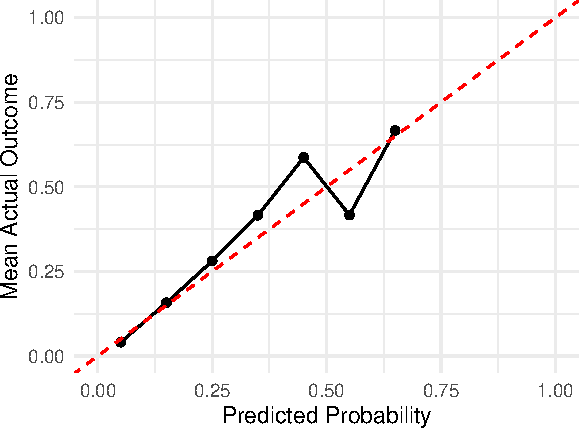
\includegraphics{Coursework_files/figure-latex/output calibration chart-1} 

}

\caption{Calibration chart for Binomial model}\label{fig:output calibration chart}
\end{figure}

We show a forest plot of the odds ratio in Figure \emph{Need code for
this} for each variable in our model. Note, it is important to state the
reference level of each factor variable, so we have a baseline for
comparison among other levels. The intercept (roughly 0.25) can be
interpreted as the probability of being a smoker if all factor variables
are at their reference level. Any blue variables, i.e.~age, imd and
urban, increase the probability by a scale of its corresponding odds
ratio and all red variables are associated with a decreased probability
of being a smoker.

\emph{Limitations of model -}

\subsubsection{Which lifestyle habits are associated with systolic blood
pressure?}\label{which-lifestyle-habits-are-associated-with-systolic-blood-pressure}

\emph{I will do this tomorrow!}

\begin{figure}[H]

{\centering 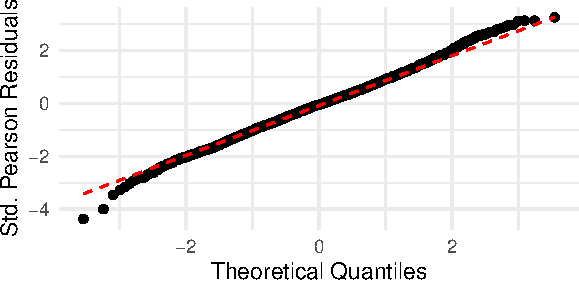
\includegraphics{Coursework_files/figure-latex/output qq plot for q3-1} 

}

\caption{Q-Q plot of Inverse-Normal model residuals}\label{fig:output qq plot for q3}
\end{figure}

\begin{figure}[H]
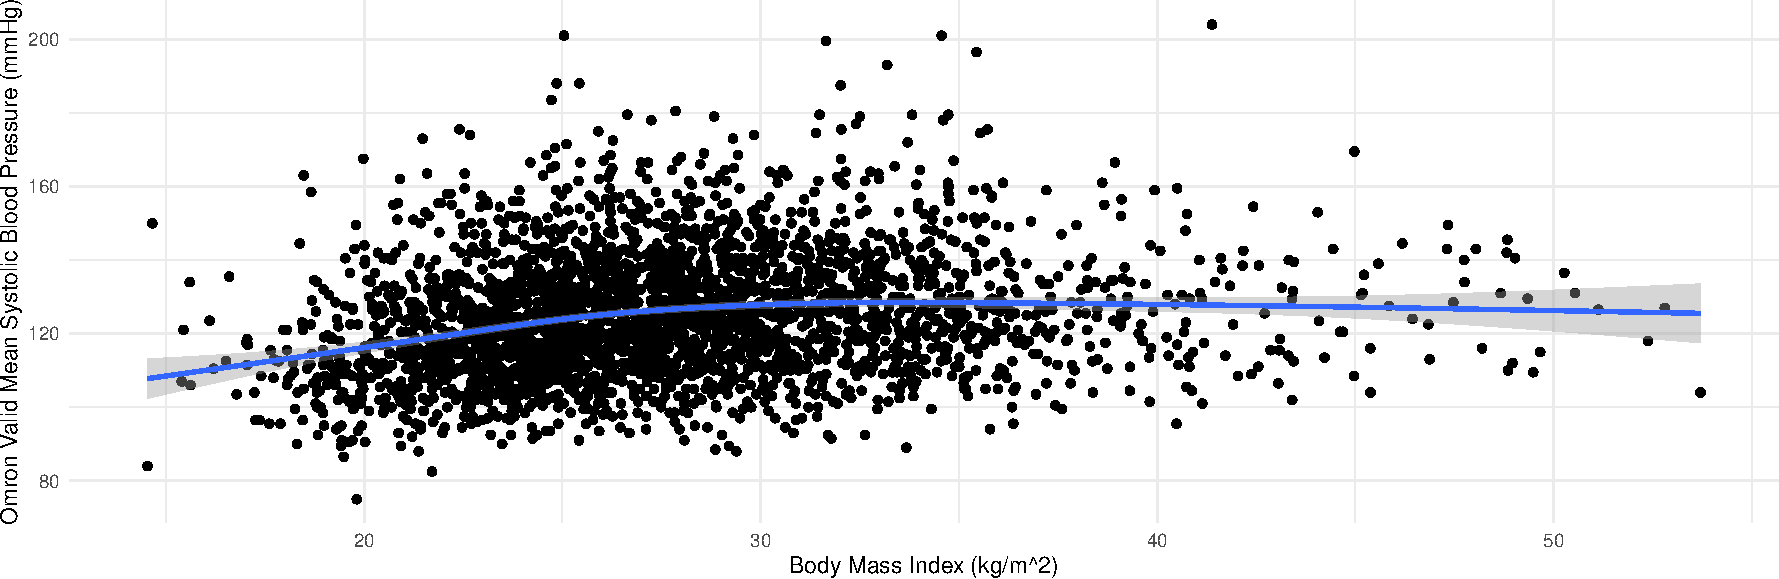
\includegraphics{Coursework_files/figure-latex/output relationship plots-1} \caption{Relationship of BMI and Age with Mean Systolic Blood Pressure}\label{fig:output relationship plots}
\end{figure}

\subsection{Results/Conclusion}\label{resultsconclusion}

Our analysis showed that alcohol consumption is extremely common among
UK adults, with approximately 81.8\% being consumers, while smoking and
vaping rates are lower at 16.7\% and 4.4\%, respectively. Older males
show the highest tendencies for alcohol consumption, with `frequent'
drinking the most prevalent among males aged 65-74. Unlike `frequent'
alcohol consumption, the prevalence of smoking decreases with age.
Individuals aged 16-24 appear to be the worst offenders when it comes to
smoking cigarettes, indicating a significant issue within youth culture.
Moreover, we found an interesting relationship between deprivation
levels and smoking and drinking behaviours. Smoking prevalence seemed to
increase as deprivation levels decrease, while alcohol consumption
appeared to do the opposite.

To help us uncover the underlying socio-economic factors that may drive
the prevalence of smoking, we first looked at the most `comparable'
respondent type in our dataset. This `respondent' is a white, single
male who has no qualifications and lives in an urban area. We found that
the probability of our hypothetical respondent being a smoker is
approximately 25\% \emph{Where is this from?} (notably higher than the
population average of 16.7). \emph{Maybe worth talking about confidence
intervals here - is value outside 95\%} The only socio-economic
variables to certainly increase this probability is the deprivation
level our respondent falls under. The rest of the socio-economic
variables we have access to, appear to decrease the likelihood of
smoking. For example, if our respondent is any of the following: Asian,
black, married, or went on to further education, the chances of them
being a smoker is at-least halved.

NatCen Social Research and Health (\citeproc{ref-Main}{2019}) \emph{?}

\newpage

\section*{References}\label{references}
\addcontentsline{toc}{section}{References}

\phantomsection\label{refs}
\begin{CSLReferences}{1}{0}
\bibitem[\citeproctext]{ref-GovUK}
GOV.UK. 2014. {``{Tax on shopping and services}.''}
\url{https://www.gov.uk/tax-on-shopping/alcohol-tobacco}.

\bibitem[\citeproctext]{ref-Main}
NatCen Social Research, Department of Epidemiology, University College
London, and Public Health. 2019. {``{Health Survey for England}.''}
\url{http://doi.org/10.5255/UKDA-SN-8860-1}.

\bibitem[\citeproctext]{ref-1ONS}
ONS. 2019a. {``{Adult smoking habits in the UK: 2019}.''}
\url{https://shorturl.at/qQW27}.

\bibitem[\citeproctext]{ref-2ONS}
---------. 2019b. {``{Alcohol-specific deaths in the UK: registered in
2019}.''} \url{https://shorturl.at/gqxY1}.

\end{CSLReferences}

\end{document}
